\setcounter{ex}{0}
% --- CÂU 1 ---
\begin{ex}
	Cho tam giác $ABC$ có $\cos A = \dfrac{4}{5}$ và $\cos B = \dfrac{5}{13}$. Tính $130\cos C - 1$.
	\shortans[oly]{31}
	\loigiai{
		Vì $A, B$ là các góc trong tam giác và $\cos A > 0, \cos B > 0$ nên $A, B$ là hai góc nhọn ($\sin A > 0, \sin B > 0$). Ta có:
		\begin{align*}
			\sin A &= \sqrt{1 - \cos^2 A} = \sqrt{1 - \left(\dfrac{4}{5}\right)^2} = \dfrac{3}{5}, \\
			\sin B &= \sqrt{1 - \cos^2 B} = \sqrt{1 - \left(\dfrac{5}{13}\right)^2} = \dfrac{12}{13}.
		\end{align*}
		Trong tam giác $ABC$, ta có $A + B + C = \pi \implies C = \pi - (A + B)$, suy ra:
		$$\cos C = \cos\left[\pi - (A + B)\right] = -\cos(A + B) = \sin A\sin B - \cos A\cos B.$$
		Thay số vào ta được:
		$$\cos C = \dfrac{3}{5}\cdot\dfrac{12}{13} - \dfrac{4}{5}\cdot\dfrac{5}{13} = \dfrac{36 - 20}{65} = \dfrac{16}{65}.$$
		Vậy:
		$$130\cos C - 1 = 130 \cdot \dfrac{16}{65} - 1 = 2 \cdot 16 - 1 = 31.$$
	}
\end{ex}

% --- CÂU 2 ---
\begin{ex}
	Cho tam giác $ABC$. Biết $\sin A + \sin B + \sin C = k\cos\dfrac{A}{2}\cos\dfrac{B}{2}\cos\dfrac{C}{2}$, tìm $k$?
	\shortans[oly]{4}
	\loigiai{
		Trong tam giác $ABC$, ta có $A + B + C = \pi \implies \dfrac{A + B}{2} = \dfrac{\pi}{2} - \dfrac{C}{2}$, do đó $\sin\dfrac{A + B}{2} = \cos\dfrac{C}{2}$ và $\cos\dfrac{A + B}{2} = \sin\dfrac{C}{2}$.\\
		Áp dụng công thức biến đổi tổng thành tích và công thức nhân đôi:
		\begin{align*}
			\sin A + \sin B + \sin C &= 2\sin\dfrac{A + B}{2}\cos\dfrac{A - B}{2} + 2\sin\dfrac{C}{2}\cos\dfrac{C}{2} \\
			&= 2\cos\dfrac{C}{2}\cos\dfrac{A - B}{2} + 2\cos\dfrac{A + B}{2}\cos\dfrac{C}{2} \\
			&= 2\cos\dfrac{C}{2}\left(\cos\dfrac{A - B}{2} + \cos\dfrac{A + B}{2}\right) \\
			&= 2\cos\dfrac{C}{2} \cdot 2\cos\dfrac{A}{2}\cos\dfrac{B}{2} \\
			&= 4\cos\dfrac{A}{2}\cos\dfrac{B}{2}\cos\dfrac{C}{2}.
		\end{align*}
		Đồng nhất với vế phải, ta tìm được $k = 4$.
	}
\end{ex}

% --- CÂU 3 ---
\begin{ex}
	Từ một vị trí $A$, người ta buộc hai sợi cáp $AB$ và $AC$ đến một cái trụ cao $15\text{ m}$, được dựng vuông góc với mặt đất, chân trụ ở vị trí $D$. Biết $CD = 9\text{ m}$ và $AD = 12\text{ m}$. Tìm góc nhọn $\alpha = \widehat{BAC}$ tạo bởi hai sợi dây cáp đó, đồng thời tính gần đúng $\alpha$ (làm tròn đến hàng phần chục, đơn vị độ).
	\begin{center}
		\begin{tikzpicture}[scale=0.35, font=\footnotesize, >=stealth]
			% Mặt đất gạch chéo
			\fill[pattern=north east lines, pattern color=gray!60] (-6, -1.2) rectangle (6, 0);
			\draw[thick] (-6, 0) -- (6, 0);
			
			% Tọa độ các điểm
			\coordinate (D) at (3, 0);
			\coordinate (A) at (-3, 0);
			\coordinate (C) at (3, 4.5);
			\coordinate (B) at (3, 7.5);
			
			% Cột trụ BD
			\draw[line width=2pt] (D) -- (B);
			\draw[thick] (2.7, 0) rectangle (3, 7.5);
			\foreach \y in {0.5, 1.5, ..., 7.0} {
				\draw (2.7, \y) -- (3, \y+0.4);
			}
			
			% Hai sợi dây cáp AB, AC
			\draw[thick] (A) -- (B);
			\draw[thick] (A) -- (C);
			
			% Cây minh họa bên trái
			\draw[line width=2.5pt, brown!60!black] (-4.5, 0) -- (-4.5, 2.5);
			\filldraw[fill=green!40!black, draw=black, thick] (-4.5, 4) circle (1.6);
			
			% Đường gióng kích thước
			\draw[<->, dashed] (3.8, 0) -- (3.8, 4.5) node[midway, right] {$9\text{ m}$};
			\draw[<->, dashed] (5.2, 0) -- (5.2, 7.5) node[midway, right] {$15\text{ m}$};
			\draw[<->, dashed] (-3, -1.6) -- (3, -1.6) node[midway, above] {$12\text{ m}$};
			
			% Nhãn các đỉnh
			\node[above left] at (A) {$A$};
			\node[above right] at (B) {$B$};
			\node[right] at (C) {$C$};
			\node[above right] at (D) {$D$};
		\end{tikzpicture}
	\end{center}
	\shortans[oly]{14,5}
	\loigiai{
		Xét hai tam giác vuông $ABD$ và $ACD$ vuông tại $D$:
		\begin{itemize}
			\item Trong $\triangle ABD$ vuông tại $D$: $\tan\widehat{BAD} = \dfrac{BD}{AD} = \dfrac{15}{12} = \dfrac{5}{4}$.
			\item Trong $\triangle ACD$ vuông tại $D$: $\tan\widehat{CAD} = \dfrac{CD}{AD} = \dfrac{9}{12} = \dfrac{3}{4}$.
		\end{itemize}
		Ta có $\alpha = \widehat{BAC} = \widehat{BAD} - \widehat{CAD}$. Áp dụng công thức cộng đối với hàm số tang:
		$$\tan\alpha = \tan\left(\widehat{BAD} - \widehat{CAD}\right) = \dfrac{\tan\widehat{BAD} - \tan\widehat{CAD}}{1 + \tan\widehat{BAD}\cdot\tan\widehat{CAD}} = \dfrac{\dfrac{5}{4} - \dfrac{3}{4}}{1 + \dfrac{5}{4}\cdot\dfrac{3}{4}} = \dfrac{\dfrac{2}{4}}{\dfrac{31}{16}} = \dfrac{8}{31}.$$
		Suy ra $\alpha = \arctan\left(\dfrac{8}{31}\right) \approx 14{,}5^\circ$ (hoặc theo kết quả làm tròn đến hàng phần chục là $14{,}5^\circ$).
	}
\end{ex}

% --- CÂU 4 ---
\begin{ex}
	Trên một mảnh đất hình vuông $ABCD$, bác An đặt một chiếc đèn pin tại vị trí $A$ chiếu chùm sáng phân kì sang phía góc $C$. Bác An nhận thấy góc chiếu sáng của đèn pin giới hạn bởi hai tia $AM$ và $AN$ mà ở đó $M \in BC$ và $N \in DC$ sao cho $BM = \dfrac{2}{3}BC$, $DN = \dfrac{1}{2}DC$. Góc chiếu sáng của đèn pin bằng bao nhiêu độ? (làm tròn đến độ)
	\shortans[oly]{30}
	\loigiai{
		Chọn độ dài cạnh hình vuông $ABCD$ là $1$ (đơn vị dài). Khi đó:
		$$AB = AD = 1, \quad BM = \dfrac{2}{3}, \quad DN = \dfrac{1}{2}.$$
		Xét các tam giác vuông $ABM$ (vuông tại $B$) và $ADN$ (vuông tại $D$):
		\begin{itemize}
			\item $\tan\widehat{BAM} = \dfrac{BM}{AB} = \dfrac{2}{3}$.
			\item $\tan\widehat{DAN} = \dfrac{DN}{AD} = \dfrac{1}{2}$.
		\end{itemize}
		Đặt $\alpha = \widehat{BAM}$ và $\beta = \widehat{DAN}$, ta có:
		$$\tan(\alpha + \beta) = \dfrac{\tan\alpha + \tan\beta}{1 - \tan\alpha\tan\beta} = \dfrac{\dfrac{2}{3} + \dfrac{1}{2}}{1 - \dfrac{2}{3}\cdot\dfrac{1}{2}} = \dfrac{\dfrac{7}{6}}{\dfrac{2}{3}} = \dfrac{7}{4}.$$
		Vì $\widehat{BAD} = 90^\circ$ nên góc chiếu sáng của đèn pin là $\widehat{MAN} = 90^\circ - (\alpha + \beta)$. Suy ra:
		$$\tan\widehat{MAN} = \tan\left[90^\circ - (\alpha + \beta)\right] = \cot(\alpha + \beta) = \dfrac{1}{\tan(\alpha + \beta)} = \dfrac{4}{7}.$$
		Do đó $\widehat{MAN} = \arctan\left(\dfrac{4}{7}\right) \approx 29{,}74^\circ \approx 30^\circ$.
	}
\end{ex}

% --- CÂU 5 ---
\begin{ex}
	Nếu $a, b$ là hai góc nhọn và $\sin a = \dfrac{1}{3}$; $\sin b = \dfrac{1}{2}$ thì $\cos 2(a + b)$ có giá trị bằng $\dfrac{7 - m\sqrt{6}}{n}$, $m, n \in \mathbb{Z}$ (phân số tối giản). Hãy tính giá trị của $m + 2n$.
	\shortans[oly]{40}
	\loigiai{
		Vì $a, b$ là hai góc nhọn nên $\cos a > 0$ và $\cos b > 0$. Ta có:
		\begin{itemize}
			\item $\cos a = \sqrt{1 - \sin^2 a} = \sqrt{1 - \dfrac{1}{9}} = \dfrac{2\sqrt{2}}{3}$.
			\item $\cos b = \sqrt{1 - \sin^2 b} = \sqrt{1 - \dfrac{1}{4}} = \dfrac{\sqrt{3}}{2}$.
		\end{itemize}
		Áp dụng công thức cộng:
		$$\sin(a + b) = \sin a\cos b + \cos a\sin b = \dfrac{1}{3}\cdot\dfrac{\sqrt{3}}{2} + \dfrac{2\sqrt{2}}{3}\cdot\dfrac{1}{2} = \dfrac{\sqrt{3} + 2\sqrt{2}}{6}.$$
		Theo công thức nhân đôi:
		\begin{align*}
			\cos 2(a + b) &= 1 - 2\sin^2(a + b) = 1 - 2\cdot\left(\dfrac{\sqrt{3} + 2\sqrt{2}}{6}\right)^2 \\
			&= 1 - \dfrac{2\left(3 + 8 + 4\sqrt{6}\right)}{36} = 1 - \dfrac{11 + 4\sqrt{6}}{18} = \dfrac{7 - 4\sqrt{6}}{18}.
		\end{align*}
		Đồng nhất với $\dfrac{7 - m\sqrt{6}}{n}$, ta được $m = 4$ và $n = 18$.\\
		Vậy $m + 2n = 4 + 2 \cdot 18 = 40$.
	}
\end{ex}

% --- CÂU 6 ---
\begin{ex}
	Một sợi cáp $R$ được gắn vào một cột thẳng đứng ở vị trí $A$ cách mặt đất $16\text{ m}$. Một sợi cáp $S$ khác cũng được gắn vào cột đó ở vị trí $B$ cách mặt đất $10\text{ m}$. Biết rằng hai sợi cáp trên cùng được gắn với mặt đất tại một vị trí $O$ cách chân cột $15\text{ m}$ (Hình vẽ). Số đo góc $\widehat{BOA} = \alpha$. Tìm giá trị $\alpha$ khi kết quả làm tròn đến hàng đơn vị theo đơn vị độ.
	\begin{center}
		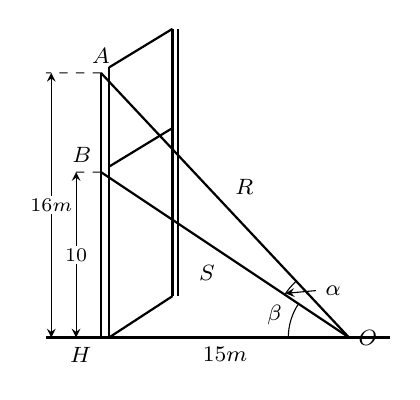
\begin{tikzpicture}[scale=0.35, font=\footnotesize, >=stealth]
			% Tọa độ
			\coordinate (H) at (0, 0);
			\coordinate (O) at (9, 0);
			\coordinate (B) at (0, 6);
			\coordinate (A) at (0, 9.6);
			
			% Mặt đất
			\draw[thick] (-2, 0) -- (10.5, 0);
			
			% Cột thẳng đứng dạng 3D nhẹ như hình gốc
			\draw[thick] (H) -- (A);
			\draw[thick] (0.3, 0) -- (0.3, 9.8);
			\draw[thick] (2.6, 1.5) -- (2.6, 11.2);
			\draw[thick] (2.8, 1.5) -- (2.8, 11.2);
			\draw[thick] (0.3, 9.8) -- (2.6, 11.2);
			\draw[thick] (0.3, 6.2) -- (2.6, 7.6);
			\draw[thick] (0.3, 0) -- (2.6, 1.5);
			
			% Hai sợi cáp R và S
			\draw[thick] (O) -- (A) node[midway, above right] {$R$};
			\draw[thick] (O) -- (B) node[midway, below left] {$S$};
			
			% Đường kích thước bên trái
			\draw[dashed] (A) -- (-2, 9.6);
			\draw[dashed] (B) -- (-1, 6);
			\draw[<->] (-1.8, 0) -- (-1.8, 9.6) node[midway, fill=white, inner sep=1pt] {\scriptsize $16\text{ m}$};
			\draw[<->] (-0.9, 0) -- (-0.9, 6) node[midway, fill=white, inner sep=1pt] {\scriptsize $10$};
			
			% Cung góc beta và alpha tại O
			\draw (O) ++(180:2.2) arc (180:146.3:2.2);
			\node at (6.3, 0.8) {$\beta$};
			\draw (O) ++(146.3:2.8) arc (146.3:133.15:2.8);
			\draw[<-] (6.7, 1.6) -- (7.8, 1.7) node[right] {$\alpha$};
			
			% Nhãn các điểm
			\node[above] at (A) {$A$};
			\node[above left] at (B) {$B$};
			\node[below left] at (H) {$H$};
			\node[right] at (O) {$O$};
			\node[below] at (4.5, 0) {$15\text{ m}$};
		\end{tikzpicture}
	\end{center}
	\shortans[oly]{13}
	\loigiai{
		Đặt $\beta = \widehat{BOH}$. Xét hai tam giác vuông $OAH$ và $OBH$ vuông tại $H$:
		\begin{itemize}
			\item Trong $\triangle OBH$ vuông tại $H$: $\tan\beta = \dfrac{BH}{OH} = \dfrac{10}{15} = \dfrac{2}{3}$.
			\item Trong $\triangle OAH$ vuông tại $H$: $\tan(\alpha + \beta) = \dfrac{AH}{OH} = \dfrac{16}{15}$.
		\end{itemize}
		Ta có $\alpha = (\alpha + \beta) - \beta$, suy ra:
		$$\tan\alpha = \tan\left[(\alpha + \beta) - \beta\right] = \dfrac{\tan(\alpha + \beta) - \tan\beta}{1 + \tan(\alpha + \beta)\tan\beta} = \dfrac{\dfrac{16}{15} - \dfrac{2}{3}}{1 + \dfrac{16}{15}\cdot\dfrac{2}{3}} = \dfrac{\dfrac{6}{15}}{\dfrac{77}{45}} = \dfrac{18}{77}.$$
		Do đó $\alpha = \arctan\left(\dfrac{18}{77}\right) \approx 13{,}15^\circ \approx 13^\circ$.
	}
\end{ex}
